\documentclass{standalone}

\usepackage{TikzStyle}
\usepackage{mystyle}

\begin{document}
    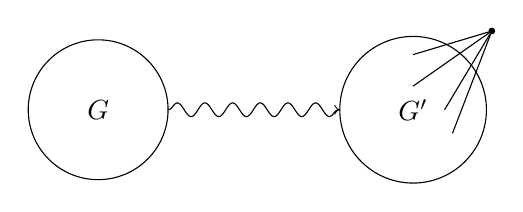
\begin{tikzpicture}
        \node[draw,circle,inner sep=0.5cm] (G) at (0,0) {$G$};
        \node[draw,circle,inner sep=0.5cm] (G1) at (4,0) {$G'$};
        \draw[->,decorate,decoration=snake] (G) -- (G1);
        \node[draw,circle,inner sep=0cm,fill=black,minimum size=2pt] (n) at (5,1) {};
        \draw (n) -- (4,0.3);
        \draw (n) -- (4,0.7);
        \draw (n) -- (4.4,0);
        \draw (n) -- (4.5,-0.3);
    \end{tikzpicture}
\end{document}
